%% equilibration_compare.tex — GENERATED by gen_equilibration_compare.py (2026-07-08).
%% Computed curves: plate-model thermal profile (50 terms, 100 Myr, L=100 km), elastic
%% equivalent density parabola (h=60 km), and their exact running integrals. Declared
%% distortions: relief (0-3 km) drawn x3; density axes broken on the water-rock blocks.
\documentclass[tikz,border=8pt]{standalone}
\usetikzlibrary{arrows.meta,patterns,patterns.meta}
\pagecolor{white}
\definecolor{cboxA}{HTML}{0072B2}   % Figure-1 trench blue
\definecolor{cboxB}{HTML}{D55E00}   % Figure-1 ridge orange
\begin{document}
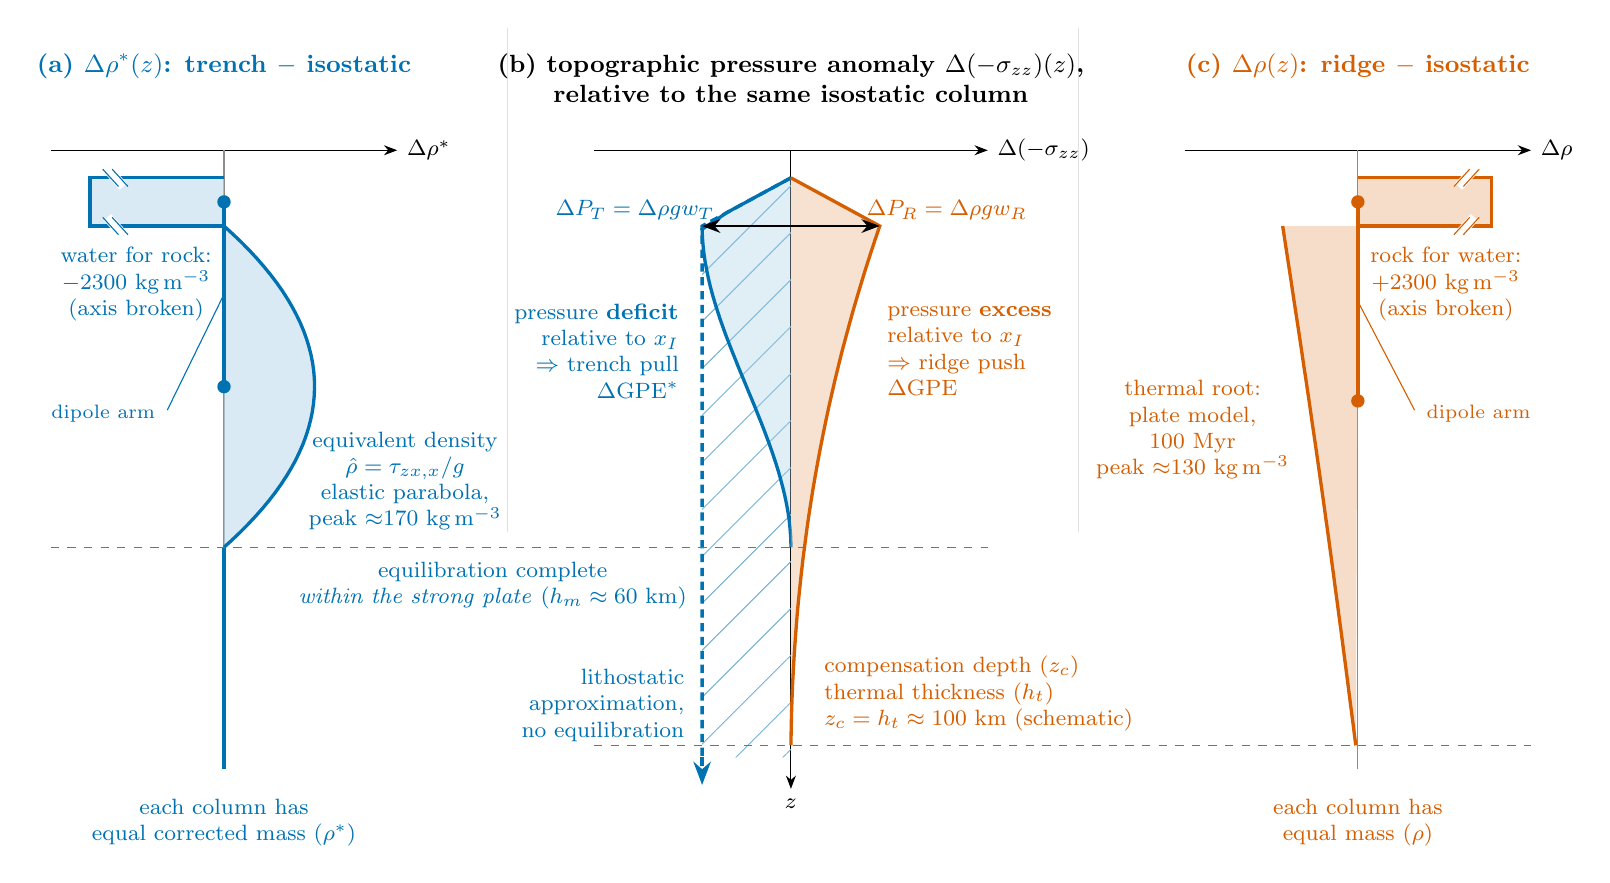
\begin{tikzpicture}[>=Stealth, font=\small,
  curveA/.style={very thick, cboxB},
  curveB/.style={very thick, cboxA},
  note/.style={font=\footnotesize, align=center},
  depthmark/.style={dashed, black!55}]

% faint separators between the three panels (drawn first, behind everything), so each comment reads as
% belonging to its own panel
\draw[black!12, line width=0.4pt] (3.6,1.9) -- (3.6,-4.5);
\draw[black!12, line width=0.4pt] (10.85,1.9) -- (10.85,-4.5);

% ============ (a) trench - isostatic: corrected density difference ============
\begin{scope}
  \node[font=\small\bfseries, cboxA, anchor=north] at (0,1.7) {(a) $\Delta\rho^{*}(z)$: trench $-$ isostatic};
  \draw[->] (-2.2,0.35) -- (2.2,0.35) node[right, font=\footnotesize] {$\Delta\rho^{*}$};
  \draw[black!45] (0,0.35) -- (0,-7.51);
  % water-for-rock block (axis broken at the cap)
  \fill[cboxA!25, opacity=0.6] (0,0) rectangle (-1.7,-0.612);
  \draw[curveB] (0,0) -- (-1.7,0) -- (-1.7,-0.612) -- (0,-0.612);
  \foreach \e in {0, -0.612} {
    \draw[white, line width=3.5pt] (-1.28,\e-0.11) -- (-1.48,\e+0.11);
    \draw[curveB, thin] (-1.22,\e-0.11) -- (-1.42,\e+0.11)
                        (-1.34,\e-0.11) -- (-1.54,\e+0.11);
  }
  \node[note, cboxA, anchor=west] at (-2.2,-1.35)
    {water for rock:\\$-2300$~kg\,m$^{-3}$\\(axis broken)};
  % elastic equivalent density parabola
  \fill[cboxA!25, opacity=0.6] plot coordinates {(0.000,-0.612) (0.113,-0.715) (0.220,-0.817) (0.321,-0.920) (0.416,-1.022) (0.505,-1.125) (0.589,-1.227) (0.667,-1.330) (0.739,-1.432) (0.805,-1.535) (0.865,-1.637) (0.920,-1.740) (0.969,-1.842) (1.012,-1.945) (1.049,-2.047) (1.080,-2.150) (1.106,-2.252) (1.126,-2.355) (1.140,-2.457) (1.148,-2.560) (1.150,-2.662) (1.146,-2.765) (1.137,-2.867) (1.122,-2.970) (1.101,-3.072) (1.074,-3.175) (1.042,-3.277) (1.004,-3.380) (0.959,-3.482) (0.910,-3.585) (0.854,-3.687) (0.792,-3.790) (0.725,-3.892) (0.652,-3.995) (0.573,-4.097) (0.488,-4.200) (0.397,-4.302) (0.301,-4.405) (0.199,-4.507) (0.091,-4.610) (0.000,-4.692)} -- (0,-0.612) -- cycle;
  \draw[curveB] plot coordinates {(0.000,-0.612) (0.113,-0.715) (0.220,-0.817) (0.321,-0.920) (0.416,-1.022) (0.505,-1.125) (0.589,-1.227) (0.667,-1.330) (0.739,-1.432) (0.805,-1.535) (0.865,-1.637) (0.920,-1.740) (0.969,-1.842) (1.012,-1.945) (1.049,-2.047) (1.080,-2.150) (1.106,-2.252) (1.126,-2.355) (1.140,-2.457) (1.148,-2.560) (1.150,-2.662) (1.146,-2.765) (1.137,-2.867) (1.122,-2.970) (1.101,-3.072) (1.074,-3.175) (1.042,-3.277) (1.004,-3.380) (0.959,-3.482) (0.910,-3.585) (0.854,-3.687) (0.792,-3.790) (0.725,-3.892) (0.652,-3.995) (0.573,-4.097) (0.488,-4.200) (0.397,-4.302) (0.301,-4.405) (0.199,-4.507) (0.091,-4.610) (0.000,-4.692)};
  \draw[curveB] (0,-4.692) -- (0,-7.51);
  \node[note, cboxA, anchor=west] at (0.95,-3.85)
    {equivalent density\\$\hat\rho=\tau_{zx,x}/g$\\elastic parabola,\\peak $\approx$170~kg\,m$^{-3}$};
  \node[note, cboxA, anchor=north] at (0,-7.76) {each column has\\equal corrected mass ($\rho^{*}$)};
  % the dipole, schematically: two equal-mass lobes and the arm between their centroids
  \draw[cboxA, very thick] (0,-0.306) -- (0,-2.652);
  \fill[cboxA] (0,-0.306) circle (0.085);
  \fill[cboxA] (0,-2.652) circle (0.085);
  \draw[cboxA, thin] (-0.72,-2.95) -- (0,-1.479);
  \node[note, cboxA, anchor=east, font=\scriptsize] at (-0.75,-3.0) {dipole arm};
\end{scope}

% ============ (b) centre: the topographic pressure anomaly ============
\begin{scope}[xshift=7.2cm]
  \node[font=\small\bfseries, align=center, anchor=north] at (0,1.7)
    {(b) topographic pressure anomaly $\Delta(-\sigma_{zz})(z)$,\\relative to the same isostatic column};
  \draw[->] (-2.5,0.35) -- (2.5,0.35) node[right, font=\footnotesize] {$\Delta(-\sigma_{zz})$};
  \draw[->] (0,0.35) -- (0,-7.76) node[below, font=\footnotesize] {$z$};
  % lobes (computed integrals)
  \fill[pattern={Lines[angle=45,distance=12pt,line width=0.35pt]}, pattern color=cboxA!55] (0,0) -- (-1.128,-0.612) -- (-1.128,-7.36) -- (0,-7.36) -- cycle;
  \fill[cboxA!35, opacity=0.35] plot coordinates {(0.000,-0.000) (-0.806,-0.437) (-1.128,-0.653) (-1.124,-0.756) (-1.116,-0.858) (-1.105,-0.961) (-1.090,-1.063) (-1.071,-1.166) (-1.050,-1.268) (-1.026,-1.371) (-0.999,-1.473) (-0.969,-1.576) (-0.937,-1.678) (-0.904,-1.781) (-0.868,-1.883) (-0.831,-1.986) (-0.792,-2.088) (-0.752,-2.191) (-0.711,-2.293) (-0.670,-2.396) (-0.628,-2.498) (-0.585,-2.601) (-0.543,-2.703) (-0.500,-2.806) (-0.458,-2.908) (-0.417,-3.011) (-0.376,-3.113) (-0.336,-3.216) (-0.298,-3.318) (-0.260,-3.421) (-0.225,-3.523) (-0.191,-3.626) (-0.159,-3.728) (-0.130,-3.831) (-0.103,-3.933) (-0.078,-4.036) (-0.057,-4.138) (-0.038,-4.241) (-0.023,-4.343) (-0.012,-4.446) (-0.004,-4.548) (-0.000,-4.651) (-0.000,-4.692)} -- (0,0) -- cycle;
  \draw[curveB] plot coordinates {(0.000,-0.000) (-0.806,-0.437) (-1.128,-0.653) (-1.124,-0.756) (-1.116,-0.858) (-1.105,-0.961) (-1.090,-1.063) (-1.071,-1.166) (-1.050,-1.268) (-1.026,-1.371) (-0.999,-1.473) (-0.969,-1.576) (-0.937,-1.678) (-0.904,-1.781) (-0.868,-1.883) (-0.831,-1.986) (-0.792,-2.088) (-0.752,-2.191) (-0.711,-2.293) (-0.670,-2.396) (-0.628,-2.498) (-0.585,-2.601) (-0.543,-2.703) (-0.500,-2.806) (-0.458,-2.908) (-0.417,-3.011) (-0.376,-3.113) (-0.336,-3.216) (-0.298,-3.318) (-0.260,-3.421) (-0.225,-3.523) (-0.191,-3.626) (-0.159,-3.728) (-0.130,-3.831) (-0.103,-3.933) (-0.078,-4.036) (-0.057,-4.138) (-0.038,-4.241) (-0.023,-4.343) (-0.012,-4.446) (-0.004,-4.548) (-0.000,-4.651) (-0.000,-4.692)};
  % lithostatic approximation (dashed): the deficit accumulates across the relief and then
  % NEVER equilibrates --- a vertical line, growing without bound with integration depth
  \draw[cboxA, very thick, densely dashed] (0,0) -- (-1.128,-0.612) -- (-1.128,-7.36);
  \draw[->, cboxA, very thick, densely dashed] (-1.128,-7.36) -- (-1.128,-7.71);
  \node[note, cboxA, anchor=east, align=right] at (-1.23,-6.7)
    {lithostatic\\approximation,\\no equilibration};
  \fill[cboxB!45, opacity=0.4] plot coordinates {(0.000,-0.000) (1.128,-0.612) (1.068,-0.788) (1.010,-0.965) (0.953,-1.141) (0.899,-1.318) (0.846,-1.494) (0.794,-1.671) (0.745,-1.847) (0.697,-2.024) (0.650,-2.200) (0.606,-2.377) (0.563,-2.553) (0.522,-2.730) (0.482,-2.906) (0.444,-3.083) (0.408,-3.259) (0.373,-3.436) (0.340,-3.612) (0.308,-3.789) (0.278,-3.965) (0.250,-4.142) (0.223,-4.318) (0.198,-4.495) (0.175,-4.671) (0.152,-4.848) (0.132,-5.024) (0.113,-5.201) (0.095,-5.377) (0.079,-5.553) (0.065,-5.730) (0.052,-5.906) (0.040,-6.083) (0.030,-6.259) (0.021,-6.436) (0.014,-6.612) (0.008,-6.789) (0.004,-6.965) (0.001,-7.142) (0.000,-7.208)} -- (0,0) -- cycle;
  \draw[curveA] plot coordinates {(0.000,-0.000) (1.128,-0.612) (1.068,-0.788) (1.010,-0.965) (0.953,-1.141) (0.899,-1.318) (0.846,-1.494) (0.794,-1.671) (0.745,-1.847) (0.697,-2.024) (0.650,-2.200) (0.606,-2.377) (0.563,-2.553) (0.522,-2.730) (0.482,-2.906) (0.444,-3.083) (0.408,-3.259) (0.373,-3.436) (0.340,-3.612) (0.308,-3.789) (0.278,-3.965) (0.250,-4.142) (0.223,-4.318) (0.198,-4.495) (0.175,-4.671) (0.152,-4.848) (0.132,-5.024) (0.113,-5.201) (0.095,-5.377) (0.079,-5.553) (0.065,-5.730) (0.052,-5.906) (0.040,-6.083) (0.030,-6.259) (0.021,-6.436) (0.014,-6.612) (0.008,-6.789) (0.004,-6.965) (0.001,-7.142) (0.000,-7.208)};
  % amplitudes: both topographic, set within the relief interval
  \draw[->, thick] (0,-0.612) -- (-1.128,-0.612);
  \draw[->, thick] (0,-0.612) -- (1.128,-0.612);
  \node[note, cboxA, anchor=south] at (-1.98,-0.662) {$\Delta P_T=\Delta\rho g w_T$};
  \node[note, cboxB, anchor=south] at (1.98,-0.662) {$\Delta P_R=\Delta\rho g w_R$};
  % areas = forces
  \node[note, cboxA, anchor=east, align=right] at (-1.3,-2.2) {pressure \textbf{deficit}\\relative to $x_I$\\$\Rightarrow$ trench pull\\$\Delta\mathrm{GPE}^{*}$};
  \node[note, cboxB, anchor=west, align=left] at (1.1,-2.2) {pressure \textbf{excess}\\relative to $x_I$\\$\Rightarrow$ ridge push\\$\Delta\mathrm{GPE}$};
  % depth ticks

\end{scope}

% ============ (c) ridge - isostatic: true density difference ============
\begin{scope}[xshift=14.4cm]
  \node[font=\small\bfseries, cboxB, anchor=north] at (0,1.7) {(c) $\Delta\rho(z)$: ridge $-$ isostatic};
  \draw[->] (-2.2,0.35) -- (2.2,0.35) node[right, font=\footnotesize] {$\Delta\rho$};
  \draw[black!45] (0,0.35) -- (0,-7.51);
  % rock-for-water block (axis broken at the cap)
  \fill[cboxB!30, opacity=0.7] (0,0) rectangle (1.7,-0.612);
  \draw[curveA] (0,0) -- (1.7,0) -- (1.7,-0.612) -- (0,-0.612);
  \foreach \e in {0, -0.612} {
    \draw[white, line width=3.5pt] (1.28,\e-0.11) -- (1.48,\e+0.11);
    \draw[curveA, thin] (1.22,\e-0.11) -- (1.42,\e+0.11)
                        (1.34,\e-0.11) -- (1.54,\e+0.11);
  }
  \node[note, cboxB, anchor=east] at (2.2,-1.35)
    {rock for water:\\$+2300$~kg\,m$^{-3}$\\(axis broken)};
  % plate-model thermal root (computed)
  \fill[cboxB!30, opacity=0.7] plot coordinates {(-0.955,-0.612) (-0.928,-0.788) (-0.901,-0.965) (-0.874,-1.141) (-0.847,-1.318) (-0.821,-1.494) (-0.794,-1.671) (-0.767,-1.847) (-0.740,-2.024) (-0.714,-2.200) (-0.688,-2.377) (-0.661,-2.553) (-0.635,-2.730) (-0.609,-2.906) (-0.584,-3.083) (-0.558,-3.259) (-0.532,-3.436) (-0.507,-3.612) (-0.482,-3.789) (-0.457,-3.965) (-0.432,-4.142) (-0.408,-4.318) (-0.383,-4.495) (-0.359,-4.671) (-0.335,-4.848) (-0.311,-5.024) (-0.288,-5.201) (-0.264,-5.377) (-0.241,-5.553) (-0.217,-5.730) (-0.194,-5.906) (-0.171,-6.083) (-0.148,-6.259) (-0.125,-6.436) (-0.103,-6.612) (-0.080,-6.789) (-0.057,-6.965) (-0.035,-7.142) (-0.026,-7.208)} -- (0,-0.612) -- cycle;
  \draw[curveA] plot coordinates {(-0.955,-0.612) (-0.928,-0.788) (-0.901,-0.965) (-0.874,-1.141) (-0.847,-1.318) (-0.821,-1.494) (-0.794,-1.671) (-0.767,-1.847) (-0.740,-2.024) (-0.714,-2.200) (-0.688,-2.377) (-0.661,-2.553) (-0.635,-2.730) (-0.609,-2.906) (-0.584,-3.083) (-0.558,-3.259) (-0.532,-3.436) (-0.507,-3.612) (-0.482,-3.789) (-0.457,-3.965) (-0.432,-4.142) (-0.408,-4.318) (-0.383,-4.495) (-0.359,-4.671) (-0.335,-4.848) (-0.311,-5.024) (-0.288,-5.201) (-0.264,-5.377) (-0.241,-5.553) (-0.217,-5.730) (-0.194,-5.906) (-0.171,-6.083) (-0.148,-6.259) (-0.125,-6.436) (-0.103,-6.612) (-0.080,-6.789) (-0.057,-6.965) (-0.035,-7.142) (-0.026,-7.208)};
  \node[note, cboxB, anchor=east] at (-0.75,-3.2)
    {thermal root:\\plate model,\\100~Myr\\peak $\approx$130~kg\,m$^{-3}$};
  \node[note, cboxB, anchor=north] at (0,-7.76) {each column has\\equal mass ($\rho$)};
  % the dipole, schematically
  \draw[cboxB, very thick] (0,-0.306) -- (0,-2.833);
  \fill[cboxB] (0,-0.306) circle (0.085);
  \fill[cboxB] (0,-2.833) circle (0.085);
  \draw[cboxB, thin] (0.72,-2.95) -- (0,-1.569);
  \node[note, cboxB, anchor=west, font=\scriptsize] at (0.75,-3.0) {dipole arm};
\end{scope}

% ============ shared depth lines, links, declared distortions ============
\draw[depthmark] (-2.2,-4.692) -- (9.7,-4.692);
\node[note, cboxA, anchor=north east] at (6.0,-4.752)
  {equilibration complete\\\emph{within the strong plate} ($h_m\approx60$~km)};
\draw[depthmark] (4.7,-7.208) -- (16.6,-7.208);
\node[note, cboxB, anchor=south west, align=left] at (7.5,-7.148)
  {compensation depth ($z_c$)\\thermal thickness ($h_t$)\\$z_c=h_t\approx100$~km (schematic)};
%% density -> pressure link ($g\int_0^z\,d\zeta$ arrows) removed 2026-08-14 (user): better stated in the caption.

\end{tikzpicture}
\end{document}
